
%-----------------------------------------------------------------------------%
\chapter{\babSatu}
%-----------------------------------------------------------------------------%
Bab ini menjelaskan latar belakang, permasalahan, tujuan dan ruang lingkup 
penelitian, serta sistematika penulisan tugas akhir penelitian 

%-----------------------------------------------------------------------------%
\section{Latar Belakang}
%-----------------------------------------------------------------------------%
Seiring berjalannya waktu, teknologi informasi (IT) mengalami perkembangan yang
pesat. Optimisasi perangkat keras untuk komputasi dan kemudahan mengakses merup
akan tujuan yang ingin dicapai. Pemanfaatannya pun beragam dari media hiburan multimedia, membantu dalam
pekerjaan sehari hari, berkomunikasi dengan orang lain, dan untuk bermain \textit{video game}.
Teknologi informasi sudah lama digunakan dalam penelitian, khususnya eksperimen secara virtual. Eksperimen ini memanfaatkan kemampuan komputer dalam komputasi dan menyimpan data dalam skala besar. Teknologi informasi yang memenuhi kriteria tersebut adalah \textit{supercomputer}.Namun, hal ini tidak terlepas dari kendala yang ada.Kemampuan komputasi yang tinggi (\textit{supercomputer}) menyebabkan besarnya biaya yang harus dikeluarkan dalam pengadaan \textit{supercomputer}.
Peneliti perlu meluangkan biaya diluar biaya penelitian tersebut.Selain itu, 
peneliti juga perlu memahami hal teknis terkait dengan pengoperasian \textit{supercomputer} dan juga perawatannya. Oleh karena itu, pemanfaatan teknologi \textit{cloud computing} dalam penelitian dapat dipandang sebagai suatu solusi alternatif.
\begin{figure}
	\centering
	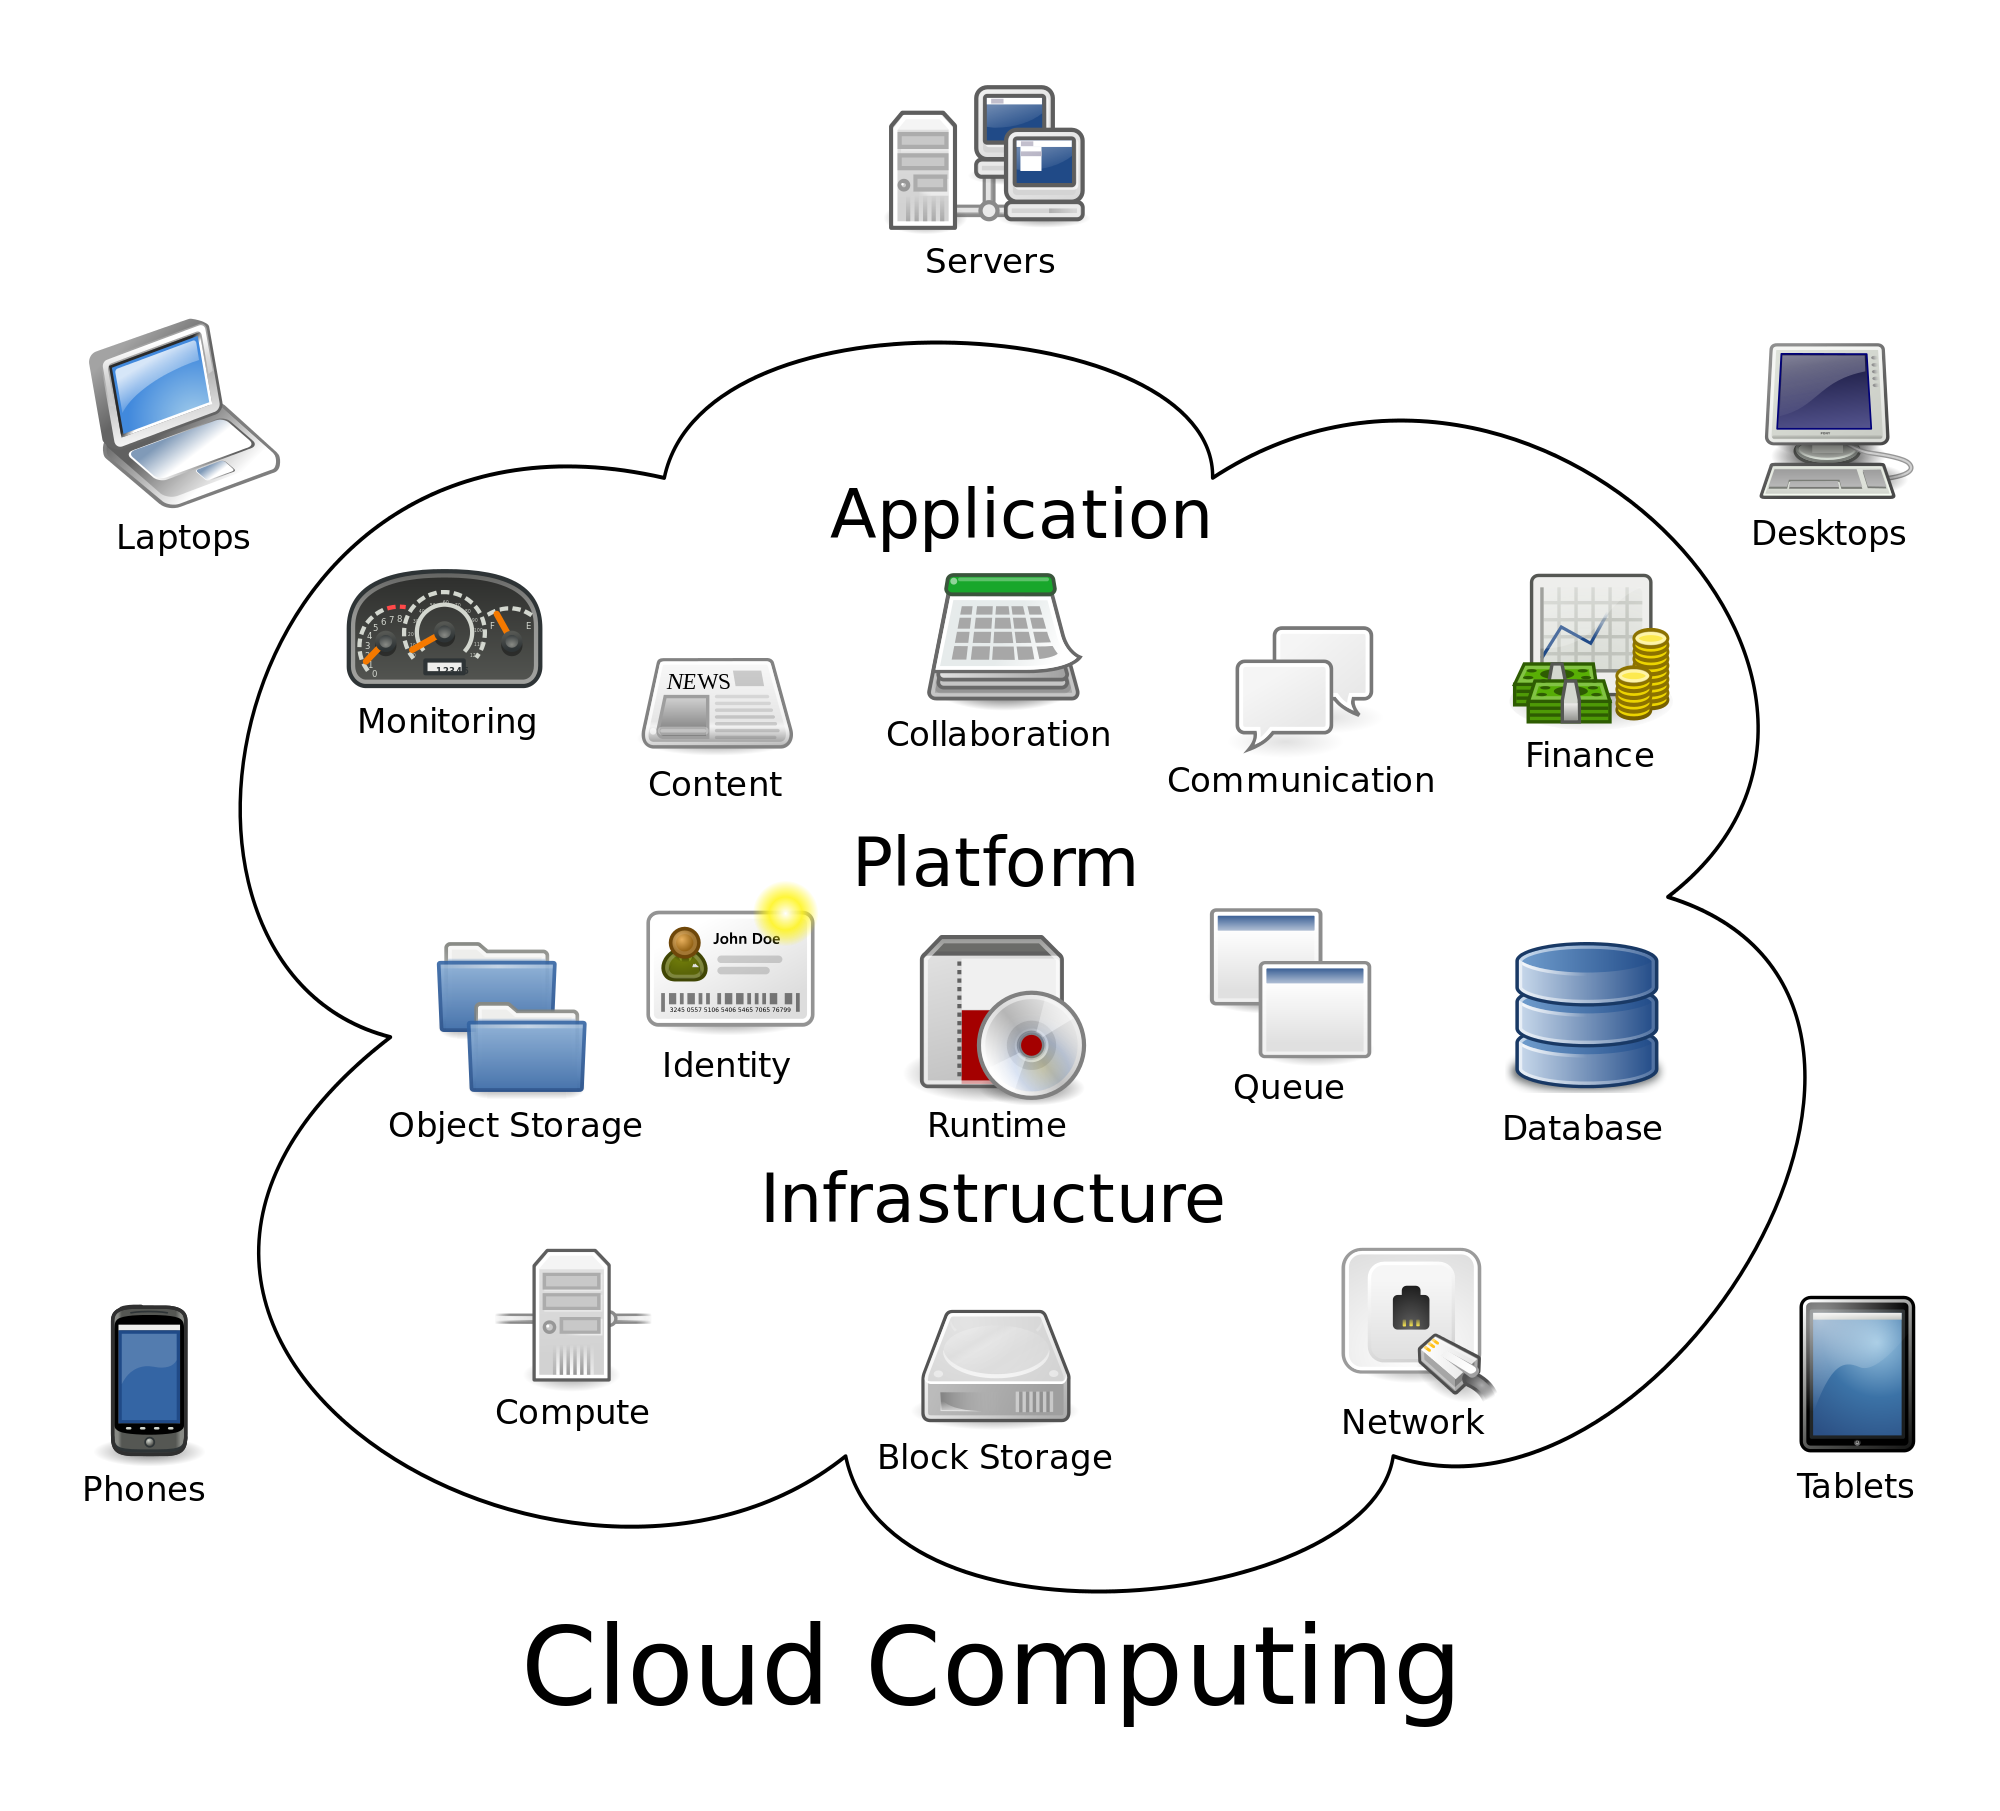
\includegraphics[scale = 0.1]{cloud_computing.png}
	\caption{Gambar 1. Ilustrasi \textit{cloud computing}}
\end{figure}
Salah satu bidang penelitian yang membutuhkan teknologi informasi dengan komputasi
tinggi adalah \textit{drug discovery}. Teknik terkait yang digunakan adalah 
\textit{virtual screening}, baik itu secara \textit{ligand-based} atau \textit{structured-based}
. Pemanfaatan teknologi \textit{cloud computing} diharapkan dapat memberikan kemudahan
bagi para peneliti tanpa perlu mempelajari secara detail pengoperasian dan perawatan teknologi yang mereka gunakan secara mendalam dan mengurangi kendala biaya dalam pengadaan \textit{supercomputer}. 

%-----------------------------------------------------------------------------%
\section{Permasalahan}
%-----------------------------------------------------------------------------%
%-----------------------------------------------------------------------------%
\subsection{Definisi Permasalahan}
%-----------------------------------------------------------------------------%
Berdasarkan latar belakang yang telah dijelaskan, penulis berusaha untuk menganalisis
apakah pemanfaatan \textit{cloud computing} dapat diajukan sebagai solusi alternatif
yang dapat digunakan oleh peneliti, khususnya terkait \textit{drug discovery}. 
Pengadaan \textit{supercomputer} akan memakan alokasi tempat maupun biaya dalam penelitian.
Selain itu, dengan adanya \textit{cloud computing}, peneliti tidak dituntut untuk memahami
teknologi terkait secara mendalam, cukup fokus dengan penelitian yang sedang dikerjakan. 
Aplikasi yang digunakan dalam tugas akhir ini adalah Docker sebagai abstraksi \textit{cluster}
komputer secara virtual seperti \textit{virtual machine} yang telah terinstall aplikasi Autodock 
dan Autodock Vina.


%-----------------------------------------------------------------------------%
\subsection{Batasan Permasalahan}
%-----------------------------------------------------------------------------%
Pada penelitian ini, penulis mencoba untuk menganalasis apakah kinerja Docker pada 
\textit{cloud computing} setara atau lebih baik dibandingkan dengan \textit{cluster} dan 
\textit{grid computing}. 


%-----------------------------------------------------------------------------%
\section{Tujuan}
%-----------------------------------------------------------------------------%
Penelitian ini secara umum bertujuan untuk mengenalkan pemanfaatan teknologi \textit{cloud computing}
sebagai alternatif pengadaan \textit{supercomputer} secara fisik khususnya \textit{drug discovery}
dalam bidang farmakologi. Selain itu, Penelitian ini secara khusus untuk menganalisis kinerja Docker
dalam menjalankan Autodock maupun Autodock Vina.


%-----------------------------------------------------------------------------%
\section{Posisi Penelitian}
%-----------------------------------------------------------------------------%
Penelitian ini merupakan .....

%-----------------------------------------------------------------------------%
\section{Sistematika Penulisan}
%-----------------------------------------------------------------------------%
Sistematika penulisan laporan adalah sebagai berikut:
\begin{itemize}
	\item Bab 1 \babSatu \\
	\item Bab 2 \babDua \\
	\item Bab 3 \babTiga \\
	\item Bab 4 \babEmpat \\
	\item Bab 5 \babLima \\
	\item Bab 6 \babEnam \\
	\item Bab 7 \kesimpulan \\
\end{itemize}

\todo{Tambahkan penjelasan singkat mengenai isi masing-masing bab.}

